\documentclass[11pt]{article}

\usepackage[a4paper,margin=2.4cm]{geometry}
\usepackage{amsmath,amssymb}
\usepackage{graphicx}
\usepackage{booktabs}
\usepackage{xcolor}
\usepackage[hidelinks]{hyperref}

\graphicspath{{../outputs/}}

\title{\textbf{Fair and Constraint-Aware Group Formation}\\[0.3em]
\large An interpretable decision-support prototype}
\author{Anastasiia Skryzhadlovska \and Matheus De Almeida Cesar Carneiro\\[0.2em]
\small University of Bologna}
\date{}

\begin{document}
\maketitle

\begin{abstract}
We design and implement a decision-support system that forms fair and balanced groups in
collaborative settings such as Erasmus+ youth exchanges. The task is modelled as a
constraint-based optimization problem: participants are partitioned into fixed-size groups
(hard constraints) so as to minimize a weighted combination of soft penalties capturing
skill balance, diversity, and preference satisfaction. We implement and compare four
methods --- a random baseline, swap-based local search, simulated annealing, and an
integer-linear-programming (ILP) formulation --- evaluate them with fairness metrics that
are deliberately independent of the optimization objective, analyse robustness under
participant addition/removal, and provide faithful per-assignment explanations. On a
synthetic cohort of $60$ participants, the optimized methods roughly halve the cost of the
random baseline; warm-started re-solving keeps assignments stable under perturbation; and a
Pareto analysis makes the skill-versus-preference trade-off explicit. We close with an
ethical discussion of fairness, inclusion, and transparency, framing the tool as support
for---not a replacement of---human judgement.
\end{abstract}

\section{Introduction}
Group composition strongly shapes inclusion, participation, and learning outcomes in
collaborative programmes. In contexts such as Erasmus+ youth exchanges, organizers must
split heterogeneous participants into balanced teams, weighing competing goals: groups
should be comparable in skill, diverse in background, and respectful of stated preferences.
Done by hand, this is slow and opaque; done na\"ively (e.g.\ at random), it is fast but
frequently unfair. Framed computationally, this is a constraint-based partitioning problem
closely related to the \emph{maximally diverse grouping problem}~\cite{mdgp} and to
team-formation tasks~\cite{teamexperts}.

This project asks how such decisions can be \emph{partially automated} while remaining
fair, robust, and interpretable. We contribute (i) a formal constraint-based model of fair
group formation; (ii) four solvers spanning heuristic and exact paradigms; (iii) an
evaluation protocol with metrics decoupled from the objective; (iv) a robustness study;
(v) a lightweight explainability layer; and (vi) an ethical analysis. The system is a
Python prototype driven from the command line, producing the figures reported here.

\section{Problem Modelling}
\label{sec:model}
Let $P=\{1,\dots,n\}$ be the participants and $\mathcal{G}=\{g_1,\dots,g_K\}$ the groups.
An \emph{assignment} is a function $\pi:P\to\mathcal{G}$.

\paragraph{Hard constraints.} Every participant belongs to exactly one group, and each
group $g$ has a fixed capacity $c_g$:
\begin{equation}
\sum_{g\in\mathcal{G}} \mathbf{1}[\pi(i)=g]=1 \quad\forall i\in P,
\qquad
\sum_{i\in P}\mathbf{1}[\pi(i)=g]=c_g \quad\forall g\in\mathcal{G}.
\end{equation}
Capacities form a balanced partition of $n$ (sizes differ by at most one). These constraints
are inviolable; an assignment satisfying them is \emph{feasible}.

\paragraph{Soft constraints.} Each soft goal is expressed as a \emph{penalty} in $[0,1]$
(lower is better), so they can be combined linearly.

Each participant $i$ has a skill vector $s_i\in[0,1]^d$. Let
$m_g=\frac{1}{|g|}\sum_{i\in g}s_i$ be the per-group skill mean. The \emph{skill-balance}
penalty is the across-group variance of these means, averaged over skills and normalized by
the maximal variance $0.25$ of values in $[0,1]$:
\begin{equation}
\Phi_{\text{skill}}(\pi)=\frac{1}{d}\sum_{j=1}^{d}
\frac{\operatorname{Var}_{g\in\mathcal{G}}\big(m_{g,j}\big)}{0.25}.
\end{equation}

For each categorical attribute $a$ (e.g.\ nationality, gender) with global distribution
$q_a$ and per-group distribution $p_{g,a}$, the \emph{diversity} penalty is the mean total
variation distance to the global mix:
\begin{equation}
\Phi_{\text{div}}(\pi)=\frac{1}{|A|\,K}\sum_{a\in A}\sum_{g\in\mathcal{G}}
\tfrac{1}{2}\sum_{c}\big|p_{g,a}(c)-q_a(c)\big|.
\end{equation}

Let $R$ be the set of directed preference relations: a \emph{like} $(i\!\to\! j)$ is
satisfied when $\pi(i)=\pi(j)$, a \emph{dislike} when $\pi(i)\neq\pi(j)$. The
\emph{preference} penalty is the unsatisfied fraction:
\begin{equation}
\Phi_{\text{pref}}(\pi)=1-\frac{|\{r\in R: r\text{ satisfied}\}|}{|R|}.
\end{equation}

\paragraph{Objective.} The optimizers minimize the weighted cost
\begin{equation}
\label{eq:cost}
C(\pi)=w_{\text{skill}}\,\Phi_{\text{skill}}(\pi)
       +w_{\text{div}}\,\Phi_{\text{div}}(\pi)
       +w_{\text{pref}}\,\Phi_{\text{pref}}(\pi),
\end{equation}
with weights $w$ encoding the organizer's priorities. Unless stated otherwise we use
$w_{\text{skill}}=1,\ w_{\text{div}}=1,\ w_{\text{pref}}=0.5$.

\section{Fairness Metrics}
\label{sec:metrics}
To avoid circular evaluation, results are judged with metrics computed \emph{independently}
of $C$: \textbf{skill imbalance} (across-group variance of group skill means, unnormalized),
\textbf{experience imbalance} (variance of per-group mean experience level),
\textbf{diversity imbalance} (mean total-variation distance, as above), and
\textbf{preference satisfaction} (the honored fraction $=1-\Phi_{\text{pref}}$). The first
three are ``lower is fairer''; the last is ``higher is better''. This separation lets a
method that games the objective be exposed by the metrics.

\section{Algorithms}
\label{sec:algorithms}
We implement four solvers spanning a random baseline, local-search
metaheuristics~\cite{localsearch,sa}, and exact constraint
programming~\cite{cp}.

\paragraph{Random baseline.} A seeded uniform feasible assignment, used as the reference
point.

\paragraph{Local search (hill climbing).} Starting from a feasible random assignment, we
repeatedly propose swapping two participants in different groups. Swaps preserve group
sizes, so feasibility is invariant. A swap is accepted iff it strictly lowers $C$; the
search stops at an iteration cap or after a no-improvement plateau. Crucially, the cost
change of a swap is evaluated \emph{incrementally}: only the two affected groups' skill
sums and category counts and the preference relations incident to the swapped pair are
recomputed, giving $O(\text{changed})$ per step rather than $O(n)$. This incremental
evaluator is verified against full recomputation in the test suite.

\paragraph{Simulated annealing (SA).} Identical machinery, but a worsening swap of cost
change $\Delta>0$ is accepted with probability $\exp(-\Delta/T)$, where the temperature $T$
is cooled geometrically~\cite{sa}. SA can escape local optima and returns the best
assignment seen.

\paragraph{Integer linear programming (ILP).} We encode binary variables $x_{i,g}\in\{0,1\}$
with the hard constraints of Section~\ref{sec:model} and solve with OR-Tools CP-SAT~\cite{ortools}. The
objective is a \emph{linear surrogate} of \eqref{eq:cost}: the preference term is exact
(same-group indicators via the linearization $z=x_{i,g}\wedge x_{j,g}$), the diversity term
is exact up to integer rounding of targets, but the skill term is an \emph{approximation} ---
variance is not linear, so we minimize the $L_1$ deviation of each group's skill total from
its balanced target. This is a faithful surrogate for \emph{balance} but a different norm
than the variance used by the metrics; we return to its consequences in
Section~\ref{sec:results}.

\section{Experimental Setup}
We generate a synthetic cohort of $n=60$ participants (seed $42$, \texttt{skewed-skill}
scenario: a minority of high performers among mostly lower-skilled participants), with $d=4$
skills, five ordinal experience levels, two diversity attributes (nationality, gender), and
optional likes/dislikes. Groups have capacity $6$ ($K=10$). Each method is run across $5$
seeds; ILP is given a $10$\,s time limit. All artifacts are regenerated by
\texttt{scripts/run\_analysis.py}.

\section{Results}
\label{sec:results}

\subsection{Method comparison}
Table~\ref{tab:methods} reports means over $5$ seeds; Figure~\ref{fig:methods} visualizes
them. The optimized methods roughly halve the cost of the random baseline. SA achieves the
lowest cost ($0.342$), with local search close behind ($0.355$) at a fraction of the
runtime. ILP attains by far the best \emph{skill} balance ($0.0008$ vs $0.003$--$0.007$),
exactly as its $L_1$ surrogate intends, but spends that advantage elsewhere: its preference
satisfaction is the lowest of the optimized methods, so its overall cost is higher. This is
the surrogate-versus-metric tension anticipated in Section~\ref{sec:algorithms}, and a
useful reminder that ``optimal'' is only optimal \emph{with respect to the encoded
objective}.

\begin{table}[h]
\centering
\caption{Mean results over 5 seeds ($n=60$, groups of 6). Lower is better except
preference satisfaction.}
\label{tab:methods}
\begin{tabular}{lrrrrrr}
\toprule
Method & Cost & Skill imb. & Exp.\ imb. & Div.\ imb. & Pref.\ sat. & Runtime (s)\\
\midrule
SA            & 0.3422 & 0.0029 & 0.1878 & 0.0900 & 0.5190 & 0.56\\
Local search  & 0.3551 & 0.0035 & 0.1844 & 0.0958 & 0.5095 & 0.19\\
ILP           & 0.4215 & \textbf{0.0008} & 0.1500 & 0.1110 & 0.3857 & 10.04\\
Random        & 0.7084 & 0.0073 & 0.3022 & 0.2830 & 0.2071 & 0.00\\
\bottomrule
\end{tabular}
\end{table}

\begin{figure}[h]
\centering
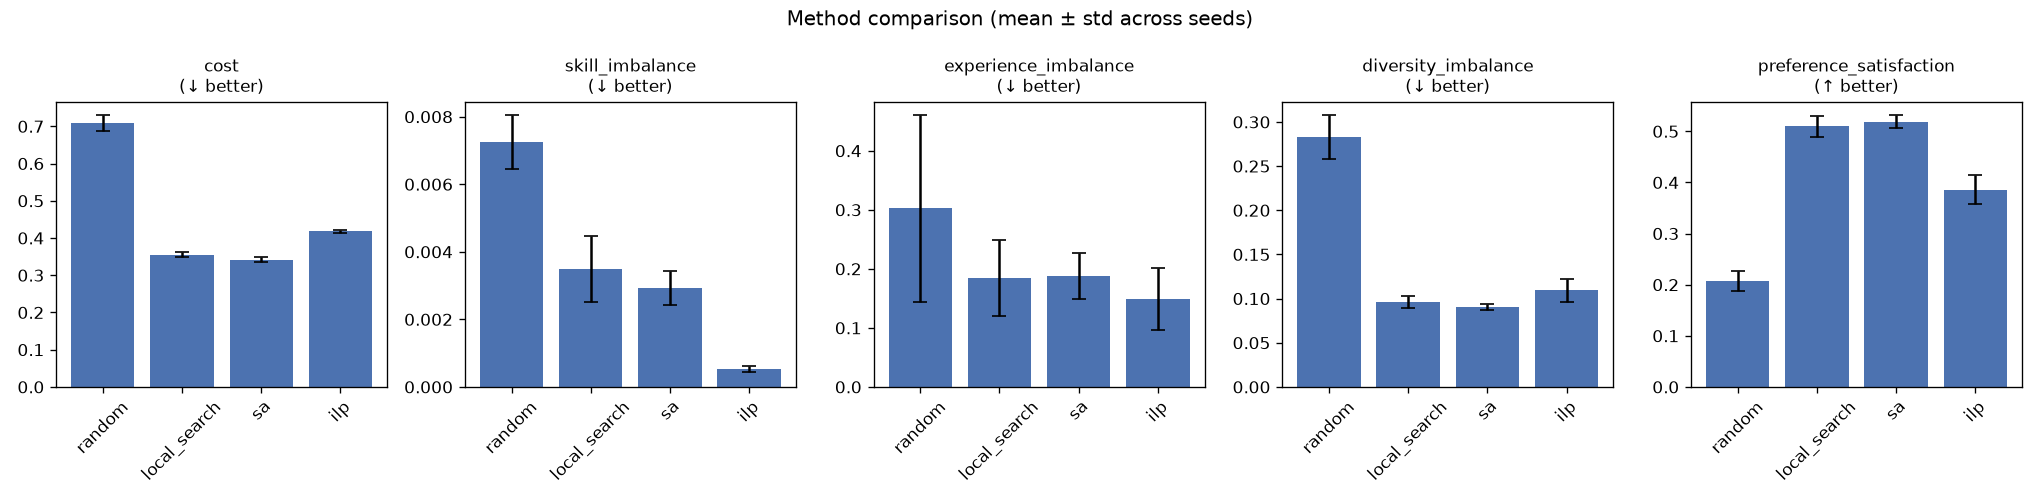
\includegraphics[width=\textwidth]{fig_method_comparison.png}
\caption{Per-metric comparison (mean $\pm$ std across seeds). Note that random achieves the
\emph{best} experience imbalance: experience is not part of the cost
\eqref{eq:cost}, so the optimizers trade it away to improve the weighted objectives.}
\label{fig:methods}
\end{figure}

A subtle but important observation in Figure~\ref{fig:methods}: the random baseline has the
\emph{lowest} experience imbalance. Because experience is not in the objective, the
optimizers freely worsen it to improve skill, diversity, and preference. This is not a bug
but a direct consequence of \emph{what we chose to optimize} --- and a concrete example of
why the metric set is broader than the objective.

\subsection{Convergence and skill distribution}
Figure~\ref{fig:conv} shows cost decreasing monotonically for hill climbing and
non-monotonically (with accepted uphill moves) for SA, which reaches a slightly lower final
cost. Figure~\ref{fig:dist} shows the spread of per-group mean skill: tight for the
optimized methods (balanced groups) and wide for random.

\begin{figure}[h]
\centering
\begin{minipage}{0.49\textwidth}
\centering
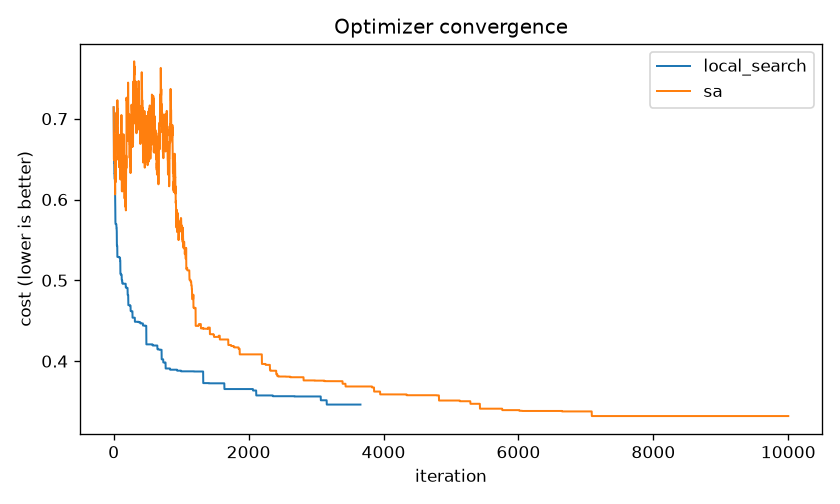
\includegraphics[width=\textwidth]{fig_convergence.png}
\caption{Cost vs iteration.}
\label{fig:conv}
\end{minipage}\hfill
\begin{minipage}{0.49\textwidth}
\centering
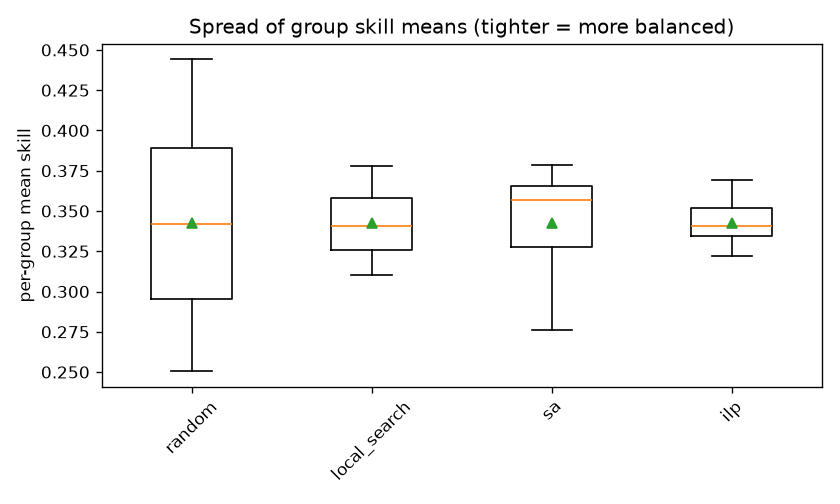
\includegraphics[width=\textwidth]{fig_skill_distribution.png}
\caption{Per-group mean skill spread.}
\label{fig:dist}
\end{minipage}
\end{figure}

\subsection{Robustness}
We perturb the cohort by removing or adding $k\in\{1,3,6\}$ participants and re-solve with
local search, comparing \emph{cold} starts (fresh random initialization) against
\emph{warm} starts (re-optimizing from the previous solution, repaired to the new
capacities). Stability is measured by the \textbf{group-change rate} (fraction of common
participants who change group, after aligning arbitrary group labels by maximum overlap)
and the label-invariant \textbf{pair-preservation} rate (fraction of participant pairs whose
same-group status is preserved). Table~\ref{tab:robust} and Figure~\ref{fig:robust}
summarize the study.

\begin{table}[h]
\centering
\caption{Mean stability over 5 trials (local search). Warm-starting drastically reduces
churn while fairness barely drifts.}
\label{tab:robust}
\begin{tabular}{llrrr}
\toprule
Perturb. & Start & $k$ & Group-change rate & Pair preservation\\
\midrule
remove & cold & 3 & 0.600 & 0.865\\
remove & warm & 3 & 0.312 & 0.918\\
add    & cold & 3 & 0.570 & 0.866\\
add    & warm & 3 & 0.107 & 0.965\\
\bottomrule
\end{tabular}
\end{table}

Warm-starting reduces the group-change rate by roughly $2$--$5\times$ relative to cold
starts (e.g.\ $0.107$ vs $0.570$ for adding three participants) while keeping
pair-preservation high. Across all settings the change in skill imbalance after perturbation
is on the order of $10^{-3}$, i.e.\ fairness is essentially preserved. For a real organizer,
this means a late change to the roster need not reshuffle everyone: warm-started re-solving
yields a stable, minimally disruptive update.

\begin{figure}[h]
\centering
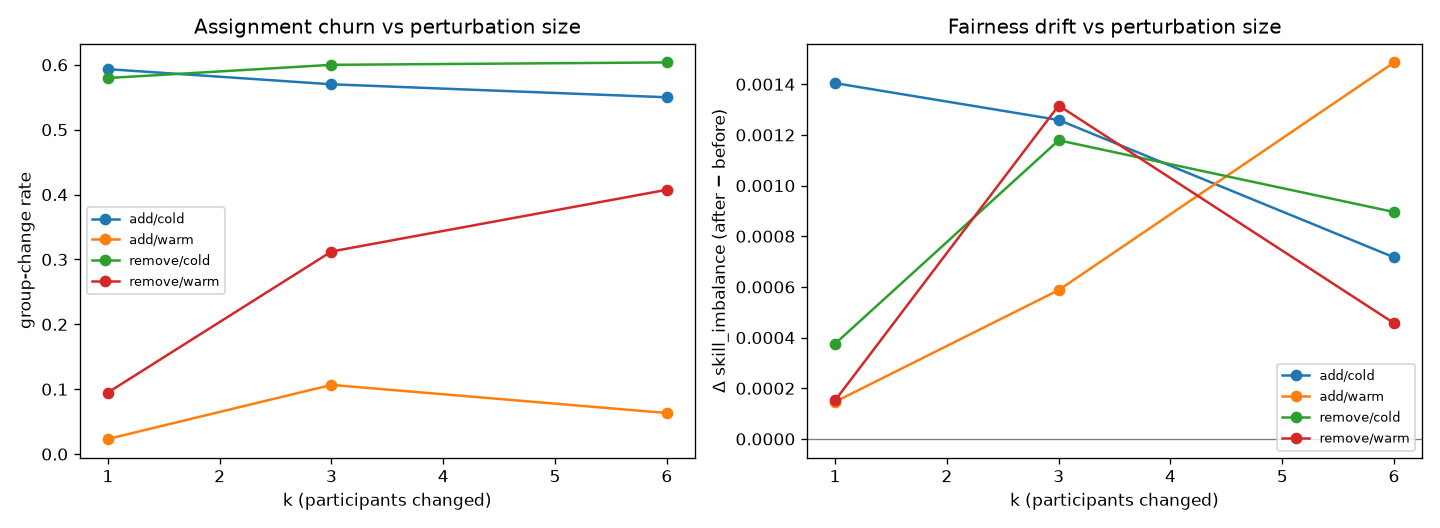
\includegraphics[width=0.95\textwidth]{fig_robustness.png}
\caption{Assignment churn (left) and fairness drift (right) vs perturbation size $k$, for
add/remove and cold/warm starts.}
\label{fig:robust}
\end{figure}

\subsection{The fairness trade-off (Pareto front)}
Soft objectives conflict: pushing skill balance can cost preference satisfaction. Sweeping
the weight $\alpha$ between skill ($w_{\text{skill}}=\alpha$) and preference
($w_{\text{pref}}=1-\alpha$) traces the trade-off in Figure~\ref{fig:pareto}. The
non-dominated (Pareto-optimal) settings lie at high $\alpha$: at $\alpha=1$ skill imbalance
is minimal ($0.00025$) but preference satisfaction collapses to $0.27$; at $\alpha=0.8$
preference satisfaction peaks ($0.64$) at a small skill cost. Notably, for $\alpha\le 0.7$
the solver converges to essentially the same solution --- the trade-off only ``bites'' near
the extremes. There is no single fair assignment: the choice along this curve is a
\emph{value judgement} that should rest with a human, which the system makes explicit rather
than hiding inside a default weight.

\begin{figure}[h]
\centering
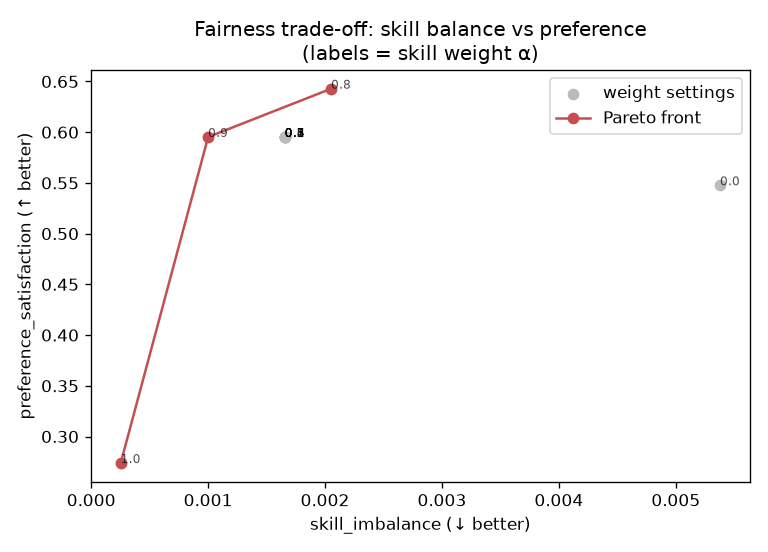
\includegraphics[width=0.7\textwidth]{fig_pareto.png}
\caption{Skill balance vs preference satisfaction as the weight $\alpha$ varies. Labels show
$\alpha$; the red curve is the Pareto front.}
\label{fig:pareto}
\end{figure}

\subsection{Explainability}
For each participant the system produces a faithful explanation grounded in the cost
model~\cite{miller}.
Because group sizes are fixed, the natural counterfactual is a \emph{swap}: we report the
single swap that would most reduce cost (using the same incremental evaluator the optimizer
uses), or state that the participant is ``well-placed'' if no swap improves the cost. On a
converged local optimum, $86\%$ of participants are well-placed. A concrete example:
\begin{quote}\small\ttfamily
Participant p007 $\rightarrow$ group g4\\
\hspace*{1em}$\bullet$ Placement: could improve by swapping with p005 (group g2, $\Delta$cost $-0.0055$)\\
\hspace*{1em}$\bullet$ Preferences: 1/2 satisfied --- grouped with liked p016; NOT grouped with liked p029\\
\hspace*{1em}$\bullet$ Diversity: nationality=PL 33\% in group vs 8\% overall (over-represented)\\
\hspace*{1em}$\bullet$ Skill: mean skill 0.27 lowers group mean 0.32 (overall 0.33)
\end{quote}
Each factor is derived from the actual soft constraints, not reconstructed post-hoc by a
separate surrogate model as in feature-attribution methods such as LIME~\cite{lime}, so the
explanation is honest about \emph{why} the placement was made and what its marginal effect
is.

\section{Ethical Discussion}
\label{sec:ethics}
Automating group formation touches directly on fairness, inclusion, and
transparency~\cite{fairml,mehrabi}.

\paragraph{Fairness is plural and contested.} Our system operationalizes fairness as a
combination of skill balance, demographic representativeness, and preference satisfaction.
These can conflict (Figure~\ref{fig:pareto})---indeed, distinct fairness criteria can be
provably impossible to satisfy simultaneously~\cite{kleinberg}---and there is no objective
``most fair'' weighting~\cite{dwork}. We therefore expose the weights as explicit, organizer-set parameters and
visualize the trade-off, rather than encoding a hidden default that would silently impose
one notion of fairness.

\paragraph{Inclusion.} Diversity is measured against the \emph{global} composition, which
spreads minorities across groups instead of concentrating them. We deliberately tested a
\texttt{minority-underrepresented} scenario; because the metric rewards matching the global
mix, a rare group tends to be distributed rather than isolated. However, when a minority is
extremely small, ``even spreading'' can also mean every such participant is the sole
representative in their group --- an outcome an organizer may or may not want. This is a
value choice the tool should surface, not decide.

\paragraph{Transparency and contestability.} Every assignment is accompanied by a faithful,
human-readable explanation and a counterfactual (Section~``Explainability''). This supports
oversight: an organizer can see why someone was placed and what the cheapest alternative is,
and can override it. Group labels are arbitrary, so we report label-invariant stability;
small wording choices like this matter for not over-claiming.

\paragraph{Decision support, not automation.} We frame the system as \emph{support} for a
human decision-maker. The optimizer encodes only what is written into the objective:
experience balance, for instance, was \emph{not} optimized and consequently degraded
(Figure~\ref{fig:methods}). This illustrates the central risk of such systems --- they
optimize precisely and only what they are told, including our blind spots --- and argues for
keeping a human in the loop who can notice unmodelled harms.

\paragraph{Limitations.} (i) Data are synthetic; real attributes carry historical bias that
a generator cannot faithfully reproduce, and naively learning ``balance'' from biased data
could entrench it. (ii) The ILP objective is a linear \emph{surrogate}; it is optimal for a
proxy, not the true metric. (iii) Reducing people to skill vectors and categorical
attributes is itself a reductive act with ethical weight. (iv) The preference model is
simple (symmetric-ish likes/dislikes) and ignores power dynamics between participants.

\section{Conclusion and Future Work}
We presented an interpretable, constraint-aware prototype for fair group formation, compared
heuristic and exact solvers, showed that optimization roughly halves the cost of random
assignment while warm-started re-solving keeps assignments stable, and made the
skill--preference trade-off explicit via a Pareto analysis. Throughout, the metric set is
broader than the objective, which exposes exactly what the optimizer neglects. Future work
includes: adding experience balance and group-level fairness floors as first-class
objectives; multi-objective optimization that returns the whole Pareto set directly;
richer, validated preference models; and a study with (consented, real) data to test whether
the synthetic findings transfer.

\paragraph{Reproducibility.} The full pipeline is regenerated by
\texttt{python scripts/run\_analysis.py}; individual steps are available as CLI commands
(\texttt{generate}, \texttt{solve}, \texttt{evaluate}, \texttt{robustness},
\texttt{pareto}, \texttt{explain}). All results above were produced with seed $42$.

\begin{thebibliography}{99}
\bibitem{mdgp} R.~R.~Weitz and S.~Lakshminarayanan. An empirical comparison of heuristic
methods for creating maximally diverse groups. \emph{Journal of the Operational Research
Society}, 49(6):635--646, 1998.
\bibitem{teamexperts} T.~Lappas, K.~Liu, and E.~Terzi. Finding a team of experts in social
networks. In \emph{Proc.\ KDD}, 2009.
\bibitem{localsearch} E.~Aarts and J.~K.~Lenstra (eds.). \emph{Local Search in Combinatorial
Optimization}. Princeton University Press, 2003.
\bibitem{sa} S.~Kirkpatrick, C.~D.~Gelatt, and M.~P.~Vecchi. Optimization by Simulated
Annealing. \emph{Science}, 220(4598):671--680, 1983.
\bibitem{cp} F.~Rossi, P.~van Beek, and T.~Walsh (eds.). \emph{Handbook of Constraint
Programming}. Elsevier, 2006.
\bibitem{ortools} L.~Perron and V.~Furnon. \emph{OR-Tools CP-SAT Solver}. Google, 2024.
\bibitem{fairml} S.~Barocas, M.~Hardt, and A.~Narayanan. \emph{Fairness and Machine
Learning: Limitations and Opportunities}. MIT Press, 2023.
\bibitem{dwork} C.~Dwork, M.~Hardt, T.~Pitassi, O.~Reingold, and R.~Zemel. Fairness through
awareness. In \emph{Proc.\ ITCS}, pp.\ 214--226, 2012.
\bibitem{kleinberg} J.~Kleinberg, S.~Mullainathan, and M.~Raghavan. Inherent trade-offs in
the fair determination of risk scores. In \emph{Proc.\ ITCS}, 2017.
\bibitem{mehrabi} N.~Mehrabi, F.~Morstatter, N.~Saxena, K.~Lerman, and A.~Galstyan. A survey
on bias and fairness in machine learning. \emph{ACM Computing Surveys}, 54(6):1--35, 2021.
\bibitem{miller} T.~Miller. Explanation in artificial intelligence: Insights from the social
sciences. \emph{Artificial Intelligence}, 267:1--38, 2019.
\bibitem{lime} M.~T.~Ribeiro, S.~Singh, and C.~Guestrin. ``Why should I trust you?'':
Explaining the predictions of any classifier. In \emph{Proc.\ KDD}, 2016.
\end{thebibliography}

\end{document}
